\documentclass[10pt]{article}
\usepackage[T1]{fontenc}
\usepackage[utf8]{inputenc}
\usepackage{lmodern}
\usepackage[margin=0.7in]{geometry}
\usepackage{amsmath,amssymb}
\usepackage{microtype}
\usepackage{enumitem}
\usepackage{graphicx}
\usepackage{float}
\usepackage[font=small,labelfont=bf,skip=3pt]{caption}
\captionsetup[figure]{font=footnotesize}
\setlength{\parskip}{2pt}
\setlength{\parindent}{0pt}
\setlist{nosep,leftmargin=*}
\setlength{\intextsep}{6pt}
\makeatletter
\renewcommand\maketitle{\begin{center}{\large\bfseries\@title\par}\end{center}}
\makeatother

\title{Why AdamW and Muon stay coupled under CE but not under MSE}

\begin{document}
\maketitle
\vspace{-0.8em}

\textbf{Answer.} Under MSE, AdamW and Muon move apart in the first hundred steps and then sit on two different
plateau functions. After that they only slowly come back together, and the shared data order never brings them
closer than two data orders of one optimizer. Under CE they also differ during the first 40 steps, but the gap shrinks
to the size of the floors by step 85. After step 221 the shared data order keeps them closer than two data orders.

\begin{itemize}
\item \textbf{Not a readout effect (measured).} With softmax$(z/T)$, where $T$ minimises the probe's cross-entropy at
each checkpoint, AdamW vs Muon is above both floors at every step after 100 (c). At step 1000 the JS is 0.30, against
0.13 for AdamW and 0.07 for Muon. At step 10{,}000 it is 0.063, against 0.060 and 0.054. Top-1 disagreement is above both
floors from step 250 on (d). The readout of Fig~1 hides the gap until about step 1250, because it puts every distance at 0.55--0.6 (b). On
the CE runs the same code reproduces Fig~1 (a; step 4000: 0.075, against 0.096 and 0.088). The L2 distance (e) cannot
decide: it shows no coupling even under CE.
\item \textbf{Not the cliff (measured).} The gap is largest on the plateau, before either optimizer reaches loss 0.9.
There it is 2 to 4.5 times the smaller floor (steps 250--1250). It shrinks after the cliff, to 1.2 times by step
10{,}000.
\item \textbf{Different solutions (measured, suggestive).} Muon's stable rank divided by AdamW's rises from 1 to 17
by step 500, while the runs separate. It then falls to 3.6, and the gap falls with it (correlation 0.94, steps
1000--10{,}000). The gap in active MLP units grows instead (correlation $-0.99$), so sparsity is not the cause. Both
series change steadily with time, so the correlation does not prove cause.
\item \textbf{Little data signal at the start (reasoned).} The MSE loss starts at 635 because the initial outputs
are large. Its gradient on the outputs is $2(z - e_y)$: the data part $e_y$ has length 1, the rest about
$\sqrt{635}\approx 25$. So for about 60 steps each optimizer mostly shrinks the outputs in its own way. That is when
the runs part: at step 62 their JS is 0.11, against floors below 0.01. Under CE the data part dominates from the first
step.
\end{itemize}

\begin{figure}[H]
\centering
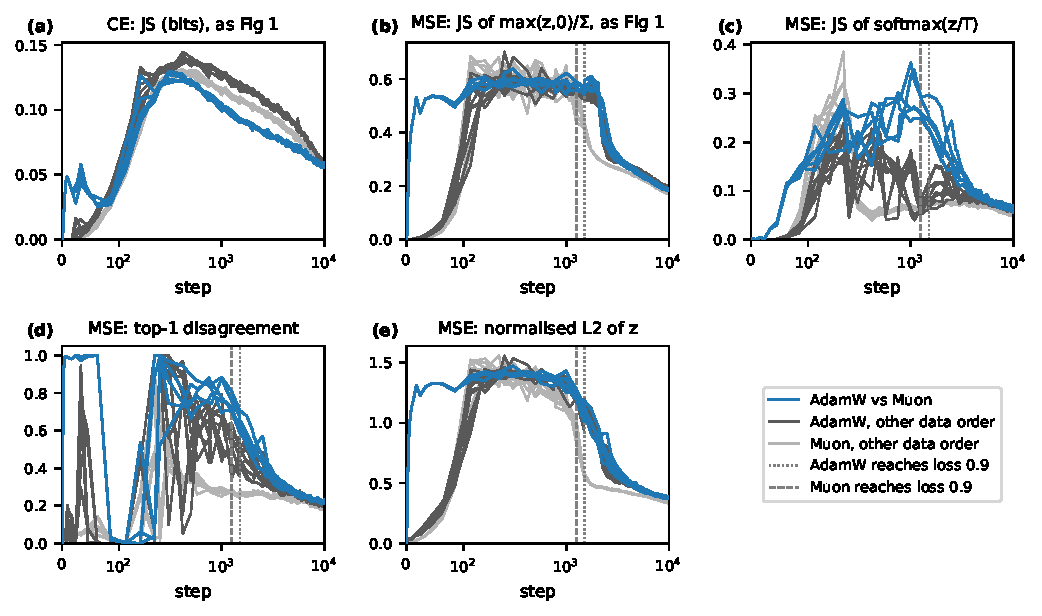
\includegraphics[width=\linewidth]{mse_paths/readouts.pdf}
\caption{Distance at equal step between AdamW and Muon on the same data order (blue), and between two data orders of
AdamW (dark grey) or Muon (light grey). (a)~CE, as in Fig~1. (b--e)~MSE under four readouts. Step axis linear up to
100, logarithmic after.}
\end{figure}

\end{document}
